\documentclass{article}
\usepackage[utf8]{inputenc}
\usepackage{natbib}
\usepackage{booktabs}
\usepackage{graphicx}
\usepackage{subfig}
\usepackage{hyperref}
\usepackage{cleveref}
\graphicspath{ {./fig/} }
\title{Global, high resolution mapping of NO2}
\author{lu et al}
\date{April 2020}

\begin{document}

\maketitle

\abstract

High-resolution (<100m) mapping of NO2 provides opportunities to study the relationship between personal air pollution exposure and health over large populations. Statistical modelling of NO2 at the global scale provides high-resolution estimations for countries with deficient ground station measurements and provides air pollution maps and human exposures with consistent uncertainties for global health studies. Our objective is to develop temporally-resolved statistical learning models, understanding the temporal dynamics of NO2 and the contributing sources, and open-source our global NO2 prediction maps at 100 m resolution. The global maps are provided at various temporal aggregations (e.g. separating between weekdays and weekends, day and night) and spatial aggregations (e.g. multiple gridded resolutions, administrative units) to facilitate global exposure assessment. To create these maps, we compiled from multiple sources a dataset of hourly NO2 measurements from more than 7000 ground stations over the globe, which is a dataset that is considerably larger in size and spatio-temporal coverage than used in recent high-resolution NO2 mapping studies. For statistical modelling, geospatial predictors include Sentinel-5 satellite (Tropomi instrument) measurements, variables relating to the emission sources (e.g., road network), dispersion processes (e.g., meteorological variables), elevation and socioeconomic indicators (i.e. VIIRS nightlight data). We evaluate various statistical models including linear models, ensemble tree-based models, deep convolution models, stacked models with regularisation, and hierarchical modelling strategies and select the optimal one for mapping. Evaluation of models includes uncertainty assessment as well as spatial validation methods. 

\section{Introduction}
Opportunities in global mapping of NO2, limitation in current studies. 
weekday and weekend, day, night: statistical predictive, exposure assessment

As NO2 varies considerably over time (e.g., between seasons), an annual estimation of NO2 and other air pollutants, as has been done in most of the classical LUR (land use regression) modeling \citep{Eeftens2012}, is unable to provide sufficient information to assess exposure when the space-time activities are considered. A relatively small number of studies developed models considering temporal variability of air pollutant concentration. \cite{BONIARDI2019108520} and \cite{CORDIOLI20171075} studying seasonal LUR models of Black carbon, PM$_x$, and common gaseous pollutants found considerable differences between warm and cold seasons.  \cite{rahman2017development} fit a LUR model to the residuals of a  periodic model of the day of the year and the day of the week to predict daily average  NO$_x$ concentrations. \cite{dons2013modeling} created a LUR model representing the diurnal cycle (hourly resolution) for Black Carbon. They developed different LUR models for each hour of the day, which has important implications in exposure studies.

Also, separation in time also affect the prediction patterns and accuracy in spatial mapping \citep{LU2020105856}.


\subsection{Main objective}
 
 \begin{enumerate}
    
\item Understanding global no2
Patterns over time, comparing the temporal patterns between difference areas.


\item
Comparison of patterns between high resolution mapping and Tropomi to understand the downscaled patterns.

\item High resolution,  temporal global NO2 map product for 2017

\end{enumerate}


 

\section{Method}
\subsection{Data}

Original data and source
\begin{verbatim}
Openstreetmap; 13 apr 2020
MERIT DEM; 90m
GHS-POP R2019A; 250m
ERA5-Land; 9km
        resolution	  nadir
Temperature	0.1 degree	10km
Wind 	    0.1 degree	10km
population	0.0025 degree 	250m
Night light	0.0042 degree	500m
radiation	0.008	800m

\end{verbatim}



buffered predictor candidates \ref{tab-buff-pred}
  
\begin{table*}\centering
\caption{buffered candidate predictors}
\label{tab-buff-pred}
\begin{tabular}{@{}lll@{}}\toprule
type & unit & buffersizes [m] \\ \midrule
roads 1 & m & 25, 50, 100, 300, 500, 1000, 3000, 5000 \\
roads 2 & m& 25, 50, 100, 300, 500, 1000, 3000, 5000 \\
roads 3 & m& 25, 50, 100, 300, 500, 1000, 3000, 5000 \\
population  &? & 1000, 3000, 5000 \\
industry  & $m^2$ & 25, 50, 100, 300, 500, 1000, 3000, 5000\\
nightlight   & ?& 450, 900, 3150, 4950\\
\bottomrule
\end{tabular}
\end{table*}

none-buffered: wind, temperature, tropomi, radiation, elevation.

\subsection{Data preprocessing}

\subsection{Modelling}
Modelling separated for each time step.

We chose XGB following...

A comparison is made with RF. 

XGB tuning

\subsection{Validation}

Accuracy matrix for weekday, weekend, day, night.

R2, RMSE, MAE, IQR

- Boostrapped CV

- Spatial cross-validation

Spatial-blocked CV,

Use Relative measures: 
R2, Relative RMSE (RMSE/median), for non-stationary NO2. 



 

\subsection{Mapping} 

\section{Result}
1. Validation result
cross validation, model interpretation, in appendix comparison with random forest
                   
2. Map
\begin{figure}
    \centering
    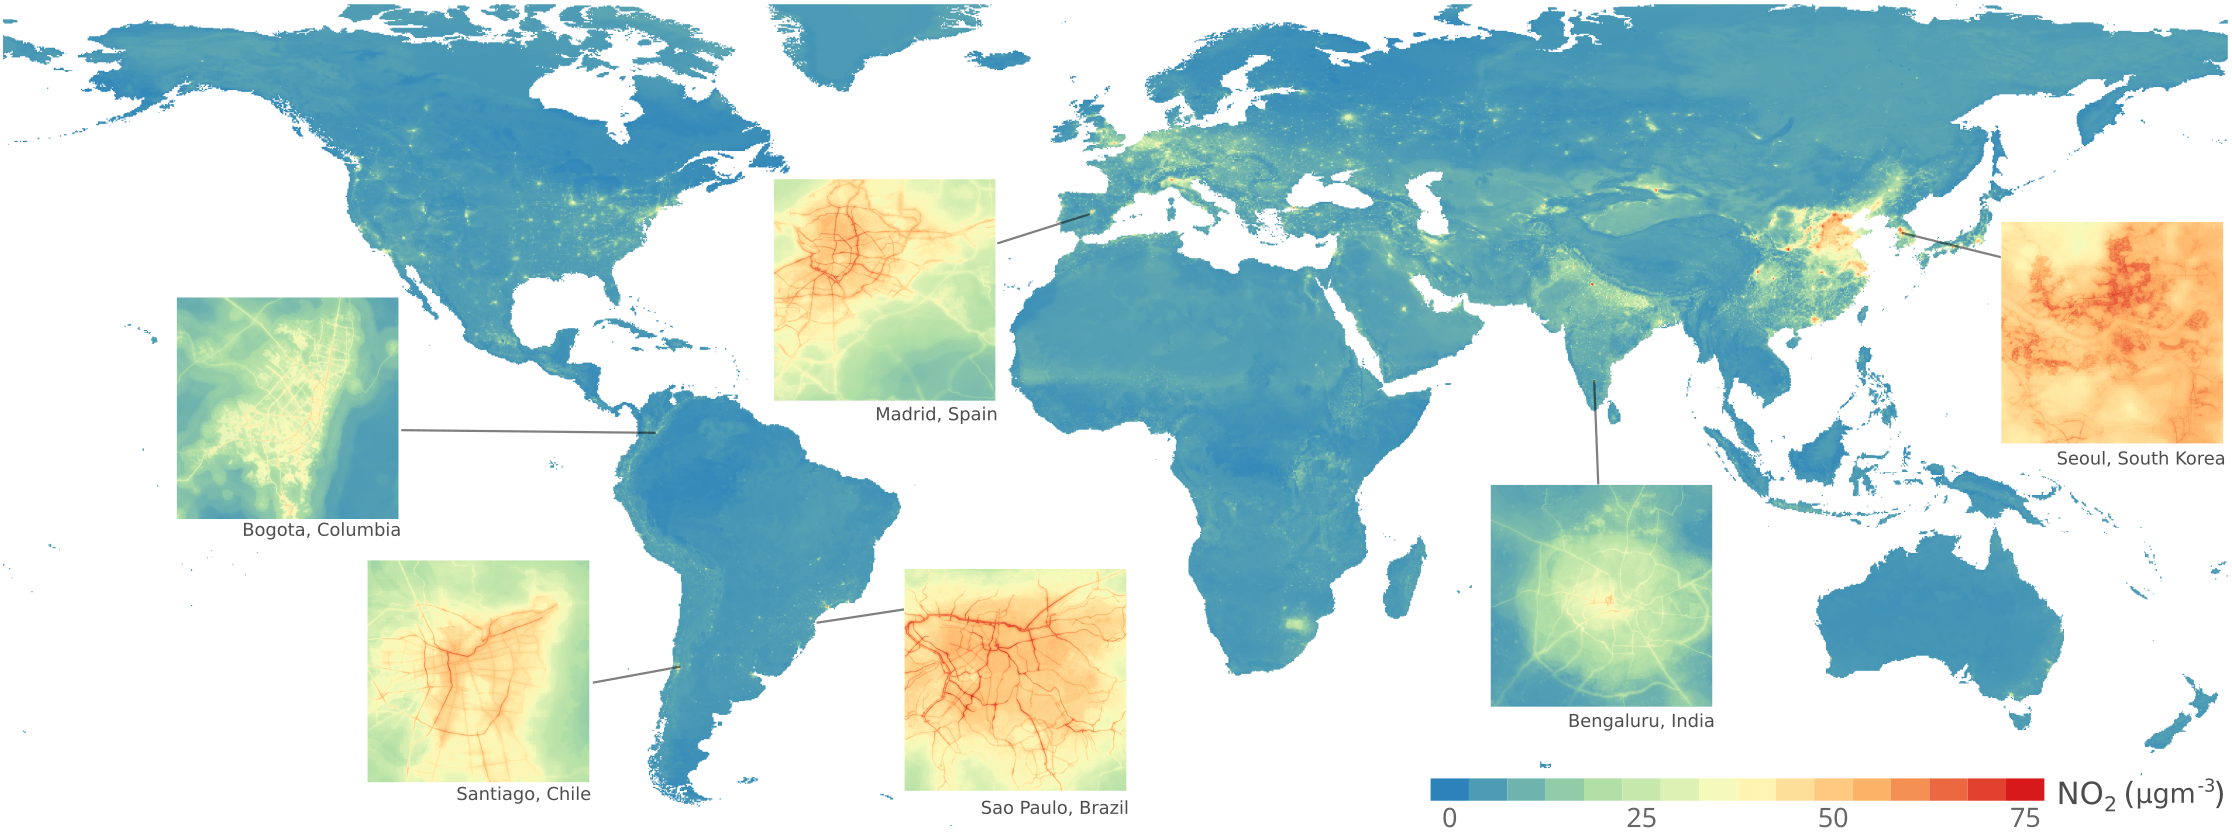
\includegraphics[width=\textwidth]{fig/glomap.png}
    \caption{global annual map, during daytime and in weekdays.}
    \label{fig:map}
\end{figure}

3. Spatial pattern in different temporal aggregations.

We show two examples in northern hemisphere and with relatively dense ground monitoring networks (\cref{fig:hamla}) and two examples in southern hemisphere and with relatively sparse ground monitoring networks (\cref{fig:adbo}). It can be observed that besides Los Angeles, USA, all examples show lower NO2 values at night times compared to the day times during weekdays. The Weekend daytime values are in general lower than the weekday daytime values. The night time values can be higher than the daytime values in some areas in weekends.   
 
\begin{figure}%
    \centering
    \subfloat[\centering Hamburg, Germany]{{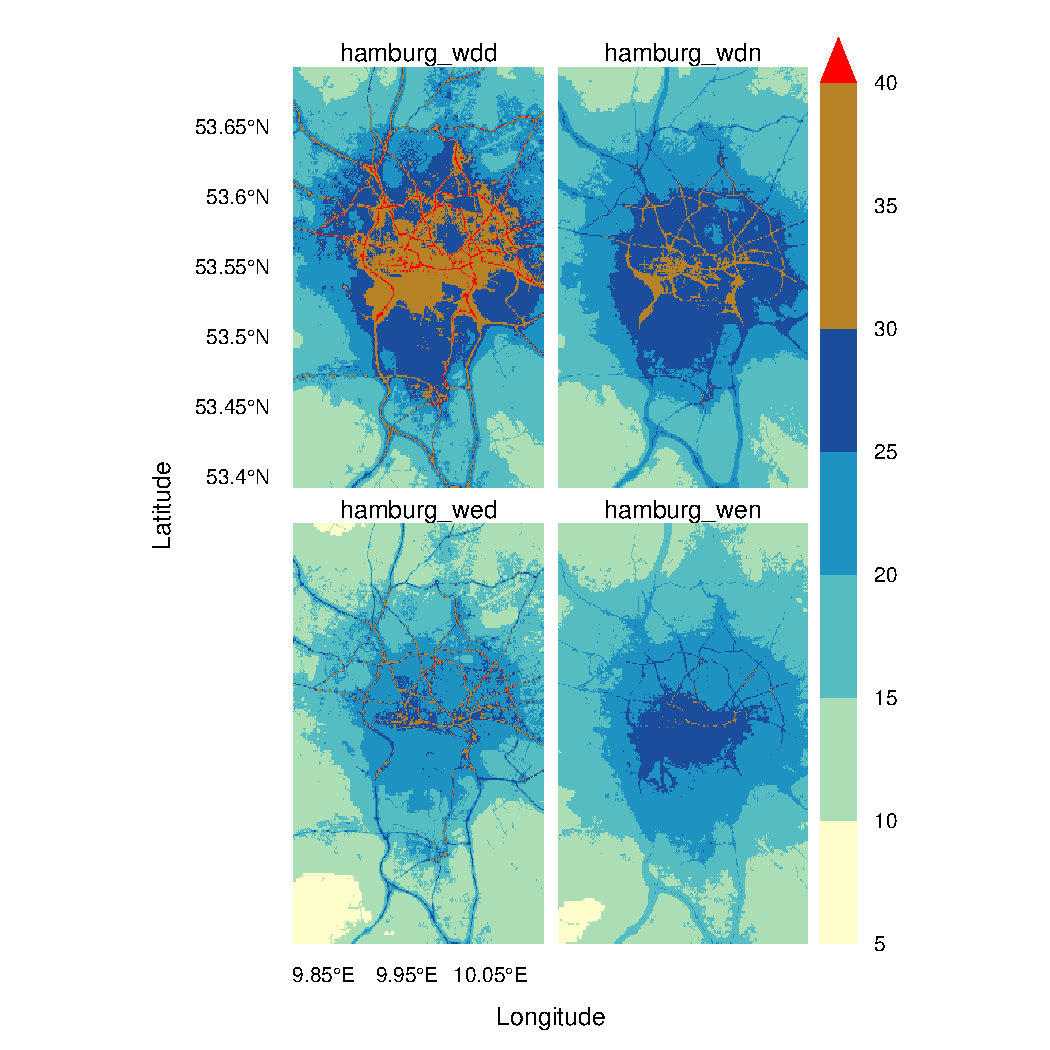
\includegraphics[width=5cm]{hamburg.pdf} }}%
    \qquad
    \subfloat[\centering Los Angeles, USA]{{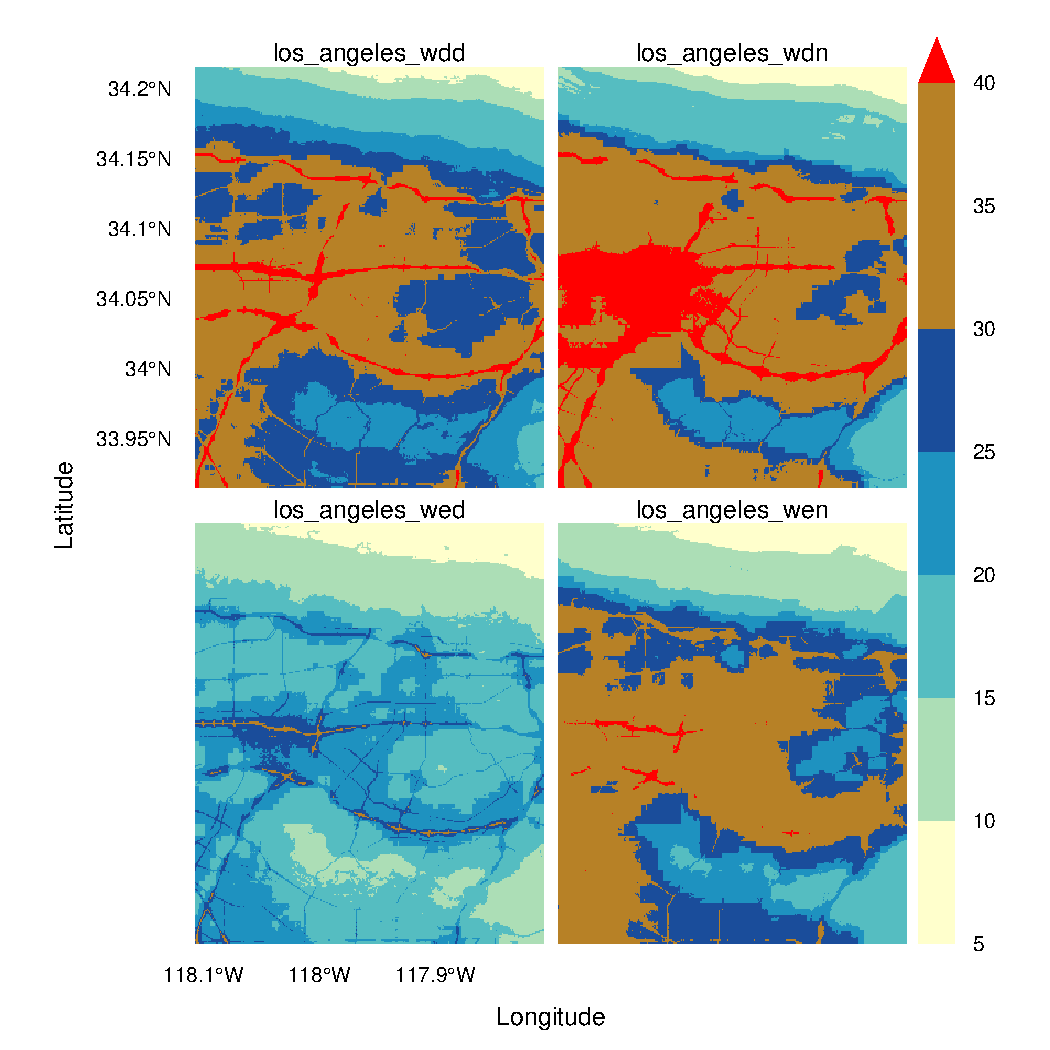
\includegraphics[width=5cm]{los_angeles.pdf} }}%
    \caption{Two examples in developed countries with relatively dense ground monitor networks.  wdd: weekday day, wdn: weekday night, wed: weekend day, wen: weekend night.}%
    \label{fig:hamla}%
\end{figure}

\begin{figure}%
    \centering
    \subfloat[\centering Addis Ababa, Euthopia]{{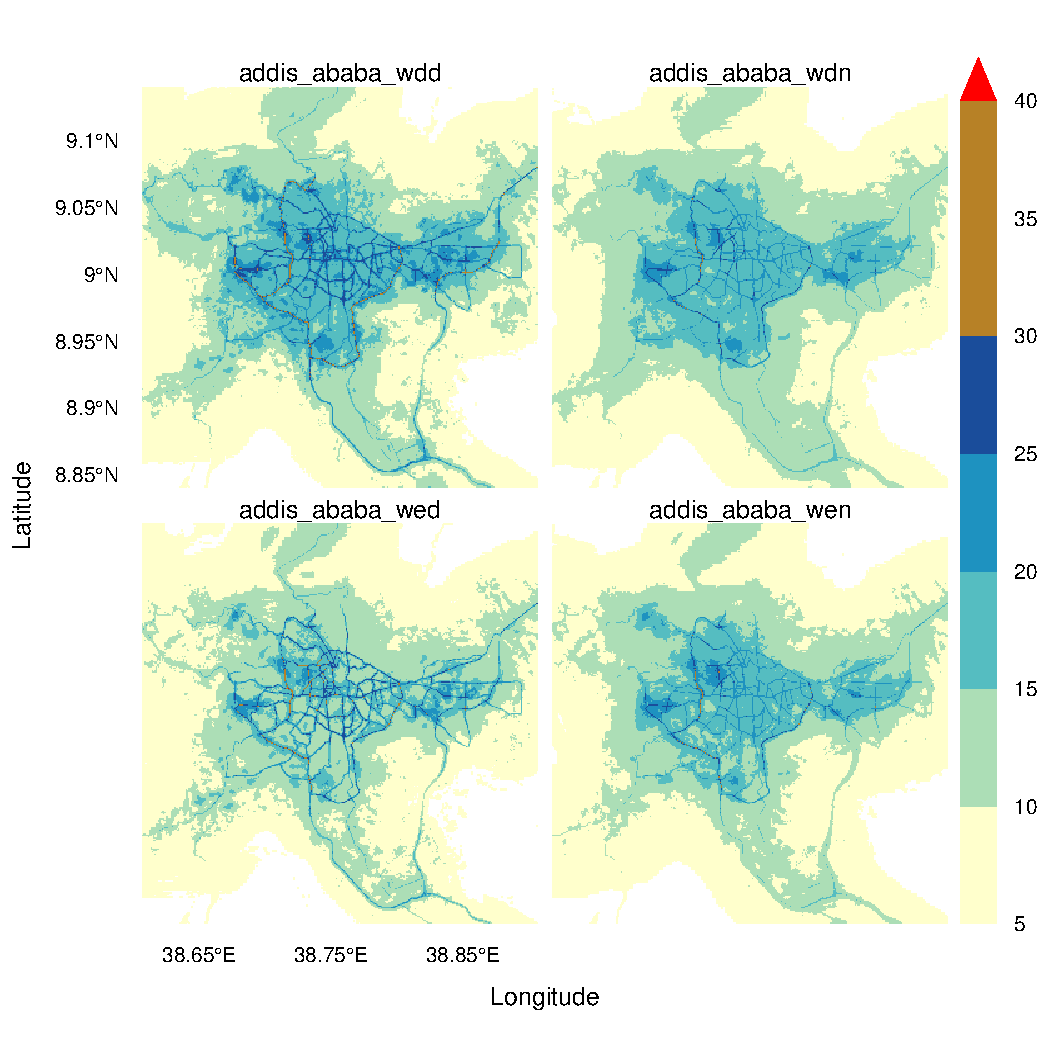
\includegraphics[width=5cm]{addis_ababa.pdf} }}%
    \qquad
    \subfloat[\centering Bogota, Columbia]{{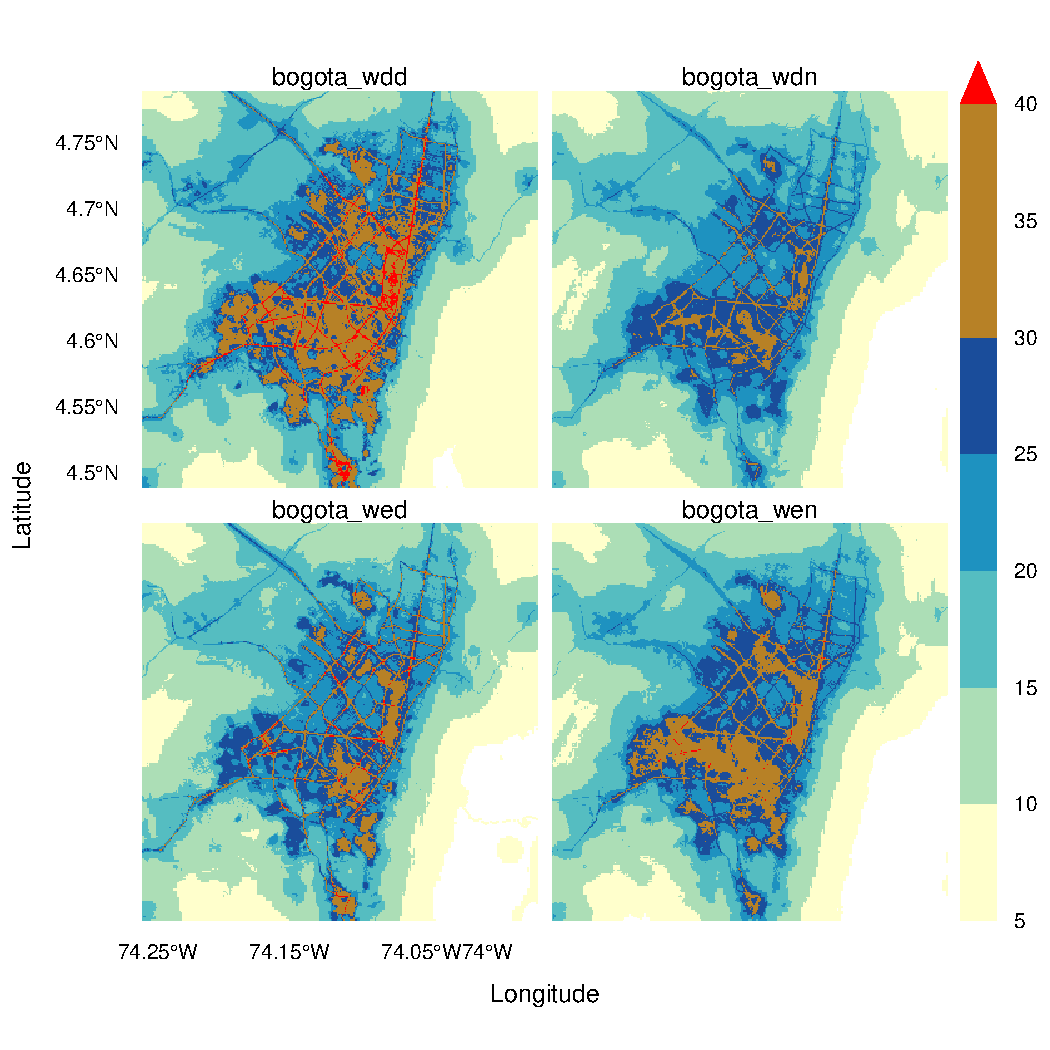
\includegraphics[width=5cm]{bogota.pdf} }}%
    \caption{Two examples in developing coutries with relatively sparse ground monitor networks.  wdd: weekday day, wdn: weekday night, wed: weekend day, wen: weekend night.}%
    \label{fig:adbo}%
\end{figure}

%4. Systematically select urban, suburban, industrial areas and compare their four temporal maps. 

4. map vs. tropomi 

Comparison with the mean in areas with dense ground station networks and with deficient measurements for comparison.



					
5, further validation: 
1)	Compare with other large-scale maps (ESCAPE or more recent maps)
2)	Other mobile sensing data, google car data? 


\section{Discussion}
Result discussion. 
Incompleteness OSM is a well-recognised issue and cannot be hidden. 

%question. where do we publish it, a web-service for viewing will greatly help with the publication. 
%The four maps in 10 km resolution with 100 m zoom in windows for details. 
%2.	On a map service, e.g. mapbox, publish the 4 maps
%3.	In a data depository, publish the predictors and 4 result maps (possibly 100m resolution)

\section{Conclusion}



 \section{To be clarified}

 1. the area (extent) of the world.   
 2. computation time
 3. all data convert back to wgs84 (4626) before merging?
 - gdal\_merge requires the same CRS for datasets to be merged. 
- we could consider to merge to 6x6 degree and publish those, similar approach is done by others
- how to publish data? (zenodo etc); creating a viewer and host?

\end{document}

\urlhttps{https://ngdc.noaa.gov/eog/viirs/download_dnb_composites.html} nightlight, 6 tiles, 2016 annual is available. 



\section{Tasks and time schedule}

Night light of 2017, monthly
NOAA/NCEI - Earth Observation Group - Defense Meteorological Satellite Progam, Boulder
"vcm-orm-ntl"
\urlhttps{https://ngdc.noaa.gov/eog/viirs/download_dnb_composites.html}

some minor updates for tomorrow based on the document and manuscript:
\begin{verbatim}
 
-M: overlap needed - all data convert back to wgs84 4626 before merging
-M: climate data has lots of missing data

\end{verbatim}
